\section{Grundlage}

\begin{frame}{Inhaltsverzeichnis}
    \tableofcontents[currentsection, hidesubsections]
\end{frame} 

\subsection{Idee}
\begin{frame}[t]{Idee}
    
\begin{itemize}
\item Physik des Jojos \pause %Erklären, was wie wir auf das Maxwell Rad gekommen sind
\begin{itemize}
\item Unterschiede: \pause %Noch ein paar Eigenschaften ergänzen
    \begin{itemize}
\item Breiter \pause
\item Keine Kraftkomponente am Boden \pause
\end{itemize}
\item Gemeinsamkeiten: \pause %Noch ein paar Eigenschaften ergänzen
\begin{itemize}
\item Faden \pause 
\item Scheibenartig 
\end{itemize}
\end{itemize}
\end{itemize}
\end{frame}

\subsection{Bilder}
\begin{frame}{Bilder}
    \begin{center}
        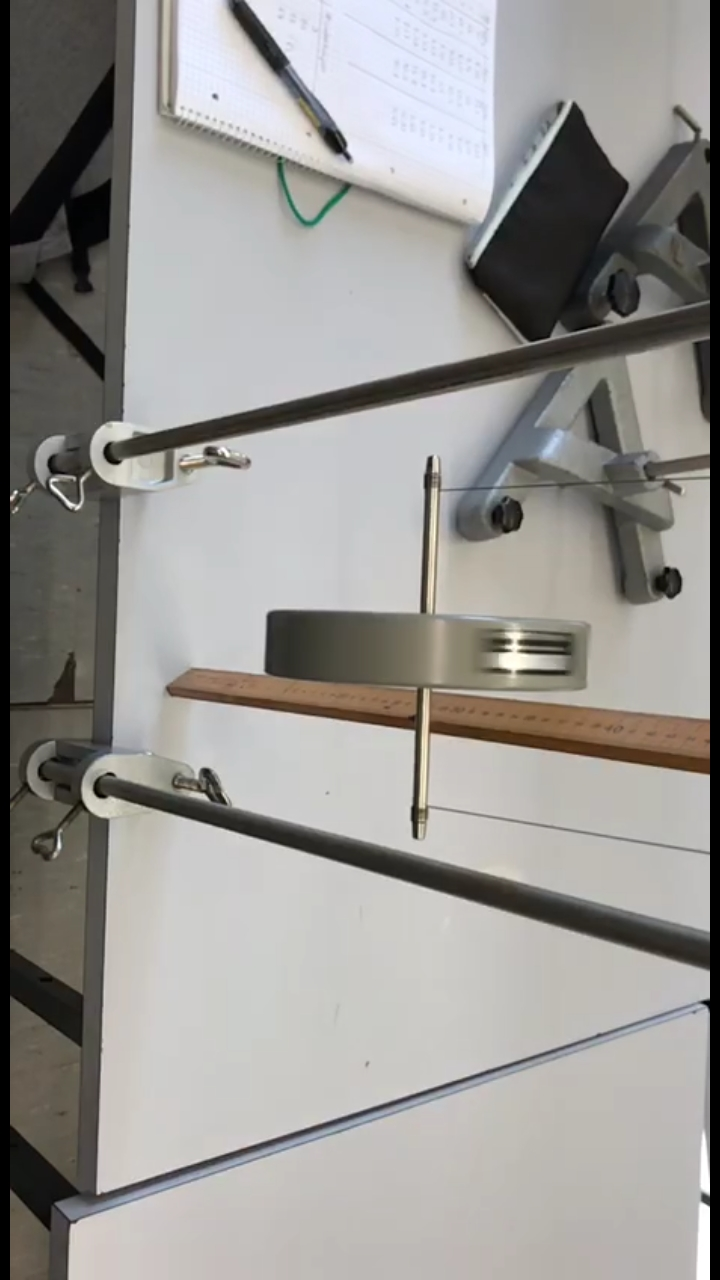
\includegraphics[width=0.2\textwidth]{build/Bild1.jpg} %Bildausrichtung usw. korrigieren
    \end{center}
\end{frame}

\begin{frame}{Bilder}
    \begin{center}
        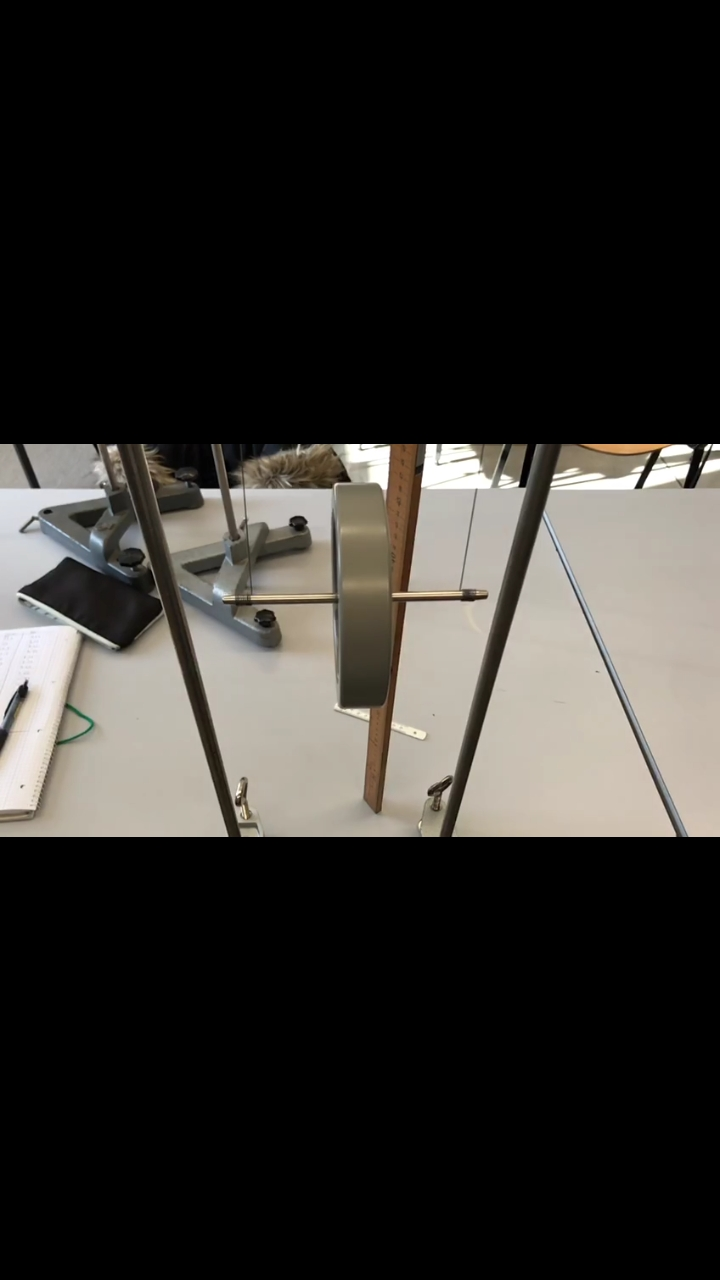
\includegraphics[width=0.2\textwidth]{build/Bild2.jpg} %Bildausrichtung usw. korrigieren
    \end{center}
\end{frame}

\subsection{Video}
\begin{frame}{Video}
    Hier ein kurzes Video unseres Versuchs:
    \begin{center}
        \movie[externalviewer]{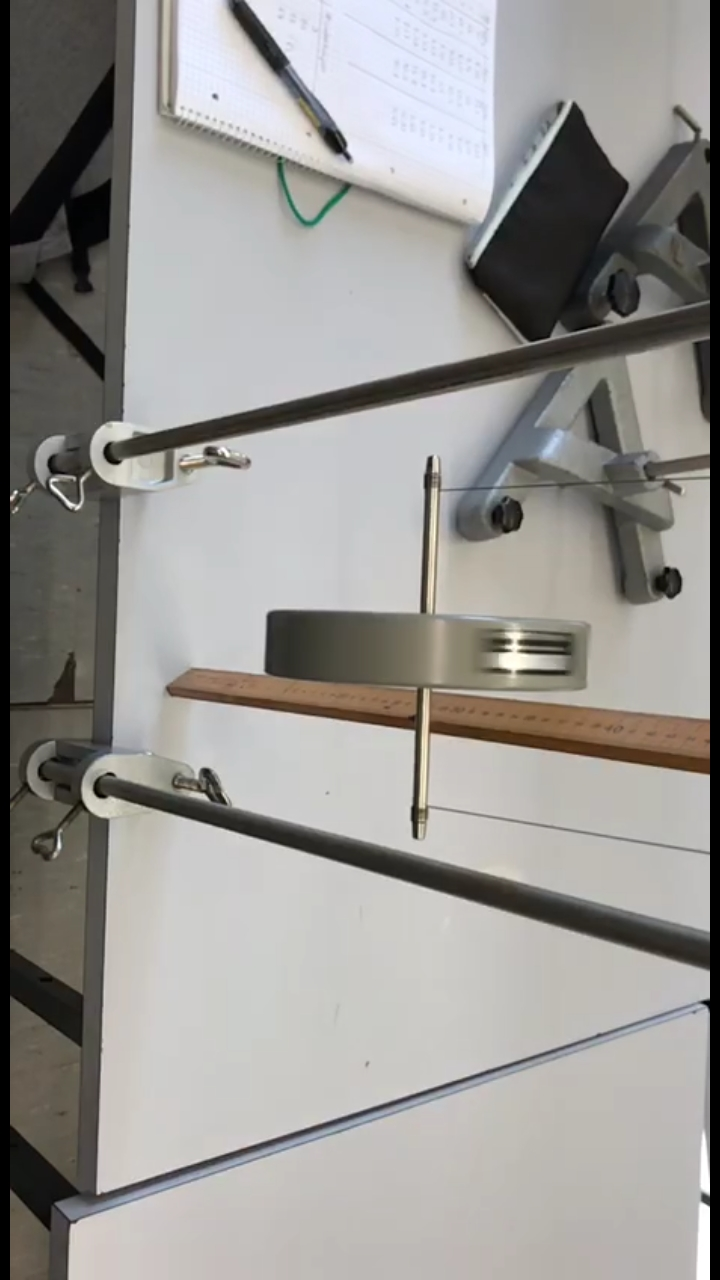
\includegraphics[width=0.2\textwidth]{build/Bild1.jpg}}{build/Video1.mp4}
    \end{center}
\end{frame}
